\documentclass[a4paper]{article}
\usepackage[a4paper,margin=0.4in,landscape]{geometry}

% default stuff
\usepackage{amsmath}
\usepackage{amssymb}
\usepackage{enumitem}

% multicolumn package
\usepackage{multicol}

\usepackage{multirow}
\usepackage{makecell}
\renewcommand\theadfont{\bfseries}

\newcolumntype{M}[1]{>{\centering\arraybackslash} m{#1}} % centered m

\newcommand{\abs}[1]{\left\lvert#1\right\rvert}

\newcommand{\ol}[1]{\begin{enumerate}#1\end{enumerate}}
\newcommand{\oll}[1]{\begin{enumerate}[leftmargin=*]#1\end{enumerate}}
\newcommand{\ul}[1]{\begin{itemize}#1\end{itemize}}
\newcommand{\ull}[1]{\begin{itemize}[leftmargin=*]#1\end{itemize}} % no margin

% coloring code
\usepackage{color}
\definecolor{dkgreen}{rgb}{0,0.6,0}
\definecolor{gray}{rgb}{0.5,0.5,0.5}
\definecolor{mauve}{rgb}{0.58,0,0.82}

\definecolor{lg}{rgb}{0.9,0.9,0.9}

% code environment
\usepackage{listings}
\lstset{
  %frame=tb, % adds top and bottom border
  aboveskip=1mm,
  belowskip=1mm,
  showstringspaces=false,
  columns=flexible,
  basicstyle={\small\ttfamily},
  numberstyle=\color{gray},
  keywordstyle=\color{blue}\textbf,
  commentstyle=\color{dkgreen},
  stringstyle=\color{mauve},
  breaklines=true,
  breakatwhitespace=true,
  tabsize=4
}
\newcommand{\ic}[1]{\lstinline{#1}}

% drawing a stack diagram
\usepackage{drawstack}
\usetikzlibrary{arrows.meta}

\newcommand{\ptr}[1]{${}^{*}$#1}
\newcommand{\addr}[1]{\&#1}
\newcommand{\addrb}[1]{(\&#1)}

% special table column for code
\usepackage{collcell}
\newcommand*{\tablecode}[1]{\lstinline{#1}}% Do anything you like with `#1`
\newcolumntype{T}{>{\collectcell\tablecode}c<{\endcollectcell}}


\graphicspath{ {./images/} }

% reduce spacing before and after headers
\makeatletter
\renewcommand{\section}{
  \@startsection{section}{1}{0pt}{1ex}{1.5ex}{\normalfont\large\bfseries}}
\renewcommand{\subsection}{
  \@startsection{subsection}{2}{0pt}{1ex}{1ex}{\normalfont\large\bfseries}}
% 5th arg is different for paragraph
\renewcommand{\paragraph}{
  \@startsection{paragraph}{4}{0pt}{1.5ex}{-0.8em}{\normalfont\bfseries}}

% line separating cols
\setlength{\columnseprule}{0.3pt}

% remove page numbering
\pagenumbering{gobble}

% skip
% L1 S44-56 (history of OS, other OS types)
% L2 S7 (memory hierarchy)
% L6 24 onwards (POSIX pthread)
% L7 41 onwards (POSIX semaphore)

\begin{document}
\begin{multicols*}{4}
  \footnotesize
  \part*{\centering \underline{CS2106}}
  \lstset{language=C}
  \section*{\underline{OS}}
    \ull {
      \item Is a program that acts as an intermediary between user and computer hardware
      \item Manages resources and coordinates requests (process synchronization, resource sharing)
      \item Simplifies programming (abstraction of hardware, convenient services)
      \item Enforces usage policies
      \item Provides security and protection (as a control program)
      \item User program portability (across different hardware)
      \item Efficiency (optimized for particular usage and hardware)
    }
    \paragraph{Kernel mode} Have complete access to all hardware resources
    \paragraph{User mode} With limited (or controlled) access to hardware resources
    \subsection*{OS types}
      \paragraph{Monolithic} Kernel is one \underline{big} special program (e.g. most Unix variants, Windows NT/XP)
        \ull {
          \item[\checkmark] Well understood; Good performance
          \item[$\times$] Highly coupled components; Usually very complicated internal structure
        }
      \paragraph{Microkernel} Kernel is \underline{small}, providing only basic essential facilities (e.g. IPC, address space \& thread management)
      \\\\
      Higher-level services (e.g. device driver, process \& memory management, file system) run as server process outside of OS, using IPC to communicate.
        \ull {
          \item[\checkmark] Kernel is more robust \& extendible; Better isolation and protection between kernel and high-level services
          \item[$\times$] Lower performance
          \item Address space refers to the set of memory locations that a program has access to
        }
      \paragraph{Layered systems} Generalization of monolithic, where components are organized into layers, which each serve a specific role
      \paragraph{Client-Server} Variation of microkernel; Client and server can be on separate machines
    \subsection*{VMs}
      \paragraph{Purpose}
        \ull {
          \item Run multiple OS on same hardware
          \item Observe inner working
          \item Test potentially destructive implementation
        }
      \paragraph{Type 1 Hypervisor}
        \ull {
          \item Runs directly on hardware (e.g. IBM VM/370)
          \item Harder to implement but better performance
        }
      \paragraph{Type 2 Hypervisor}
        \ull {
          \item Runs on host OS (e.g. VMware);
          \item Easier to implement but worse performance
          \item Independent of actual hardware, can use to emulate hardware you don't have
        }
  \section*{\underline{Process Abstraction}}
    \paragraph{Process} An abstraction to describe a running program
    \paragraph{Memory context} A process has:
      \ull {
        \item Text: for instructions
        \item Data: for global variables
        \item Heap: for dynamic allocation
        \item Stack: for function invocations
      }
      Note that pointers are stored as storing raw data is impractical (but OS must ensure that the data of switched-out process is not modified)
    \paragraph{Hardware context}
      \ull {
        \item General purpose registers (GPRs)
        \item PC, SP, FP, etc.
      }
    \paragraph{Register spilling} If GPRs are insufficient, use memory to temporarily hold GPR values
    \subsection*{Stack frame example}
      \paragraph{Executing function call}
        \oll {
          \item Pass arguments with registers and/or stack
          \item Save return PC on stack
          \item \textbf{Transfer control from caller to callee}
          \item Save registers to be used by callee. Save old FP, SP
          \item Allocate space for local vars of callee on stack
          \item Adjust SP to point to new stack top
        }
      \paragraph{Returning from function call}
        \oll {
          \item Restore saved registers, FP, SP
          \item \textbf{Transfer control from callee to caller using saved PC}
          \item Continues execution in caller
        }
      \begin{center}
        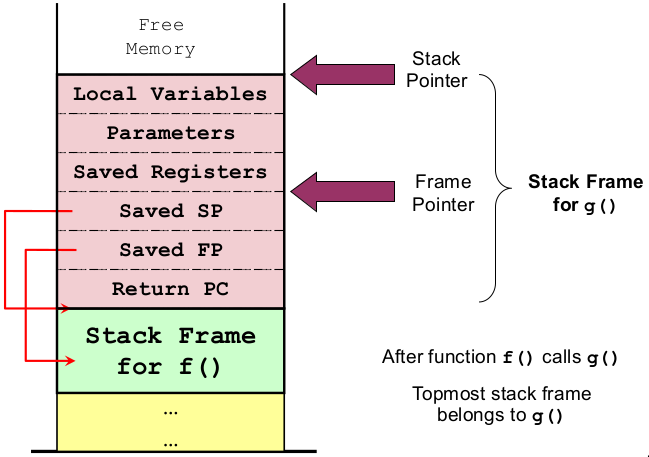
\includegraphics[width=0.24\textwidth]{stack_frame}
      \end{center}
      \paragraph{Misc}
        \ull {
          \item Saved SP is important in architectures without \ic{PUSH} and \ic{POP} instructions (where you need to load and store to address pointed at by SP)
          \item SP may change, FP stays constant
          \item Stack frame sizes may not be computable at compile time, if we use \ic{alloca} (not required for CS2106)
          \item There are scenarios where SP, FP are not required
          \item Stack teardown is achieved by modifying SP. Results stay on stack until overwritten
        }
    \subsection*{Process ID \& State}
      \paragraph{Generic 5-state process model}
        \begin{center}
          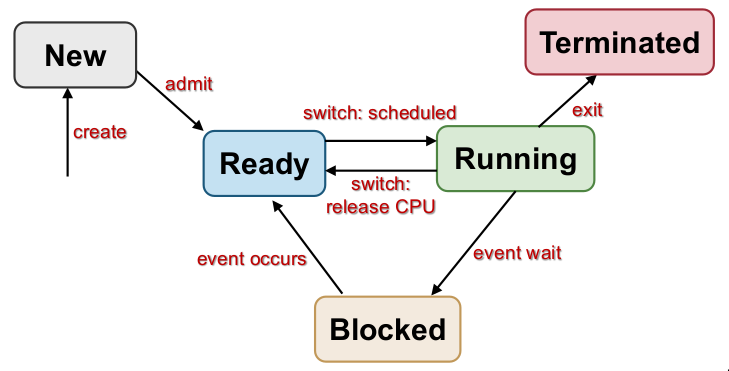
\includegraphics[width=0.24\textwidth]{process_model}
        \end{center}
      \paragraph{Process control block (PCB)} Stores the entire execution context for a process:
        \ull {
          \item Memory, hardware contexts
          \item OS context: PID, process state
        }
    \subsection*{System calls}
      \ull {
        \item Implemented as a kernel-mode routine with some parameters
      }
      \paragraph{In C/C++} Can be almost directly invoked
        \ull {
          \item Most have a library version with same name and params, acting as a function wrapper
          \item Few have a more user-friendly version with flexible params, acting as a function adapter
        }
      \paragraph{General mechanism}
        \oll {
          \item User program invokes library call
          \item Library call places syscall number in designated location
          \item Library call executes TRAP instruction to \textbf{switch from user mode to kernel mode}
          \item Appropriate syscall handler is determined, using syscall number as index (usually handled by a dispatcher)
          \item Syscall handler is executed (carries out actual request)
          \item Return control to library call, switch from kernel mode to user mode
          \item Library call returns to user program
        }
    \subsection*{Exception/Interrupt/Signal}
      \paragraph{Exception} Synchronous (occurs due to program execution)
        \ull{
          \item Executes an exception handler, like a forced function call
          \item Traps are intentionally set up exceptions
        }
      \paragraph{Interrupt} Asynchronous (occurs independent of program execution, usually hardware related)
        \ull {
          \item Executes an interrupt handler, program execution is suspended
          \item From hardware to OS kernel
        }
      \paragraph{Signal} High level communication mechanism in Unix OSes
        \ull {
          \item Asynchronous wrt program that receives them
          \item When an exception occurs, info may be delivered to a process via a signal
        }
  \section*{\underline{Process Abstraction in Unix}}
    \paragraph{Process information}
      \ull {
        \item PID (integer)
        \item Process State (running, sleeping, stopped, zombie)
        \item Parent PID
        \item Cumulative CPU time, etc.
      }
    \paragraph{C command line args}
      \ull {
        \item \ic{main} has signature \ic{int main(int argc, char* argv[])}
        \item \ic{int argc} contains the number of command line args (including program name)
        \item \ic{char* argv[]} contains the command line args as C character strings
      }
    \paragraph{Create} \ic{int fork()}
      \ull {
        \item \ic{#include <unistd.h>}
        \item Returns PID of newly created process (to parent process), and 0 (to child process)
        \item Child is basically a duplicate of parent, with the execption of PID and PPID
        \item Memory regions are copied from parent
        \item Child starts running from the immediate \textbf{machine instruction} after the fork
        \item Linux provides \ic{clone()}, a more verstaile version of \ic{fork()}, that allows specification of what execution context can be shared
        \item Running a command in a terminal is essentially a \ic{fork()} followed by \ic{exec()}
      }
    \paragraph{Fork implementation}
      \oll {
        \item Create address space of child
        \item Allocate new PID, p'
        \item Create kernel process data structures (e.g. entry in process table)
        \item Copy kernel environment of parent process (e.g. priority)
        \item Initialize child process context (PID=p', PPID=parent id, CPUtime=0)
        \item Copy memory regions from parent (expensive, can be optimized, next section)
        \item Acquires shared resources (open files, cwd)
        \item Initialize hardware context for child (copy registers, etc.)
        \item Add child to scheduler queue
      }
    \paragraph{Copy on write}
      \ull {
        \item Child potentially needs to copy the whole memory space
        \item Child might not need the entire memory space immediately
        \item If child just reads, then can use shared version
        \item Only if ANY write occurs, then must have independent copies of data
      }
    \paragraph{Execute} \ic{exec} family of calls
      \ull {
        \item \ic{#include <unistd.h>}
        \item Replaces current executing process image with new one
        \item Only code is replaced, but PID and other information stays intact
        \item Has several different variants: \ic{execl, execv, execve, excle, execvp}
        \item \ic{int execl( const char *path, const char *arg0 ... *argN, NULL )}
        \item e.g. \ic{execl("/bin/ls", "ls", "-l", NULL)}, same as executing \ic{ls -l} in terminal
      }
    \paragraph{Terminate} \ic{void exit(int status)}
      \ull {
        \item Status is returned to the parent process
        \item 0 indicates normal termination, not 0 indicates problematic execution
        \item Does not return (control flow does not go to callee), but exit status is communicated to callee
        \item Most programs have no explicit \ic{exit()} call, but returning from \ic{main()} implicitly calls \ic{exit()}.
      }
    \paragraph{Master process} \ic{init}
      \ull {
        \item Created in kernel at boot up time
        \item Traditionally has PID = 1
        \item Root process
      }
    \paragraph{On exit}
      \ull {
        \item Most system resources are released (e.g. file descriptors)
        \item Some basic resources are not releasable (e.g. PID, status - for parent-child sync; CPU time - for process accounting)
        \item Process table entry may still be needed
      }
    \paragraph{Wait} \ic{int wait(int *status)}
      \ull {
        \item Returns PID of terminated child process
        \item \ic{int *status} stores the exit status of the terminated child. Init to NULL if this info is not needed.
        \item Blocking: parent blocks until one child terminates (then removes child from process table)
          \ull {
            \item Even if child is a new executable (\ic{exec}), still waits
            \item If there are no children, does not block
          }
        \item Cleans up remainder of child system resources not removed in exit
        \item Variants: \ic{waitpid()} that waits for a specific child process, \ic{waitid()} that waits for any child process to change status
      }
    \paragraph{Zombie process}
      \ull {
        \item \ic{wait()} creates zombie processes, as the (dead) child process might need to pass information to the parent
        \item If parent terminates first, then \ic{init()} becomes the pseudo parent. Child termination sends a signal to \ic{init()} which uses \ic{wait()} to cleanup
        \item If child terminates first (and parent did not \ic{wait()}), child becomes zombie, which can fill up the process table.
        \item On older Unix implementations, may need a reboot to clear the table
        \item If parent never terminates, zombie processes will continue to exist
      }
    \paragraph{Get PID}
      \ull {
        \item \ic{pid_t} is a signed integer type, but in GNU this is an \ic{int} instead.
        \item \ic{pid_t getpid()} returns the process PID
        \item \ic{pid_t getppid()} returns the parent process PID
      }
    \paragraph{Unix process model}
      \begin{center}
        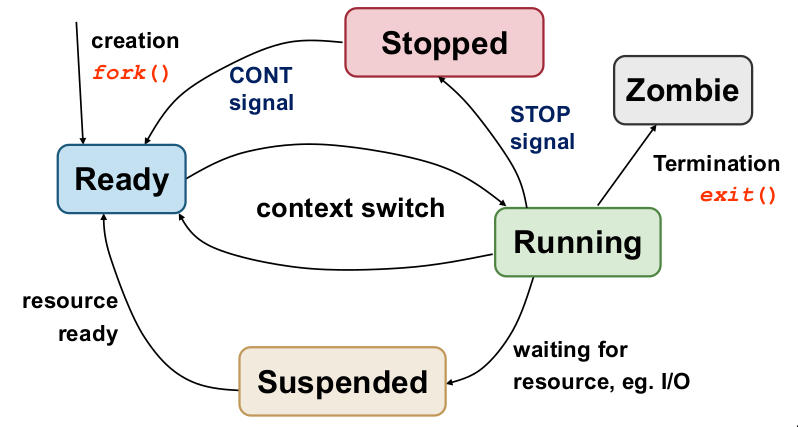
\includegraphics[width=0.24\textwidth]{process_model_unix}
      \end{center}
  \section*{\underline{Process scheduling}}
    \ull {
      \item When does the OS/scheduler run?
        \ull {
          \item Woken up by events (e.g. data arrival, timer interrupt, process termination)
          \item Save context of running process
          \item Do what OS needs to do
          \item Restore context
        }
      \item I/O signals are handled by interrupt service routines (not user-space processes)
      \item If there is only 1 process, the scheduler let it run without intervening (save on overhead and context switching)
    }
    \paragraph{Non-preemptive}
      \ull {
        \item Process stays scheduled until it blocks, or gives up CPU voluntarily
        \item Lesser overhead
      }
    \paragraph{Preemptive}
      \ull {
        \item At the end of the time quota, the process is suspended (a process might still block or finish/give up CPU early)
        \item Used when responsiveness of system is important
      }
    \paragraph{CPU/Compute-bound} Process spends most of its time using CPU
    \paragraph{IO-bound} Process spends most of its time using I/O
    \subsection*{Batch processing}
      No user interaction, non-preemptive scheduling is predominant
      \paragraph{Criteria}
        \ull {
          \item Throughput: Number of tasks finished per unit time
          \item Turnaround time: Total wall clock time (finish - start), includes waiting time
          \item CPU utilization: Percentage of time when CPU is working
        }
      \paragraph{First come first served (FCFS)}
        \ull {
          \item Maintain a FIFO queue based on arrival time
          \item Blocked task is removed from queue, and placed at back once it is ready
          \item Non-preemptive
          \item No starvation: number of tasks before X in FIFO is always decreasing
          \item Simple reordering can reduce average waiting time (cf. SJF)
        }
      \paragraph{Convoy effect}
        \ull {
          \item CPU-bound task A is followed by many IO-bound tasks $X_1, X_2, \cdots, X_N$
          \item Task A runs, while tasks $X_i$ wait in ready queue (I/O is idle)
          \item Task A blocked on I/O, so tasks $X_i$ execute on CPU quickly, now blocked on I/O (CPU is idle)
        }
      \paragraph{Shortest Job First (SJF)}
        \ull {
          \item Select task that takes shortest amount of CPU time
          \item Need to know total CPU time for a task in advance. Common approach is exponential average:
            \[ \text{Predict}_{t+1} = \alpha \text{Actual}_t + (1-\alpha) \text{Predict}_t \]
            \ull {
              \item $\alpha$ represents the significance of the immediate past value
              \item $1 - \alpha$ represents the significance of the past history
            }
          \item Can be preemptive or non-preemptive
          \item Starvation is possible; biased towards short jobs
        }
      \paragraph{Shortest Remaining Time (SRT)}
        \ull {
          \item Preemptive version of SJF, using remaining CPU time
          \item New job with shorter remaining time can preempt currently running job
          \item If all tasks arrive at beginning, SRT gives same schedule as SJF
          \item Starvation is possible
        }
    \subsection*{Interactive systems}
      \paragraph{Criteria}
        \ull {
          \item Response time: Time between request and response by system
          \item Predictability: Variation in response time (important in real-time environments)
          \item Interval of timer interrupt (ITI): OS scheduler is triggered every ITI (typically 1ms to 10ms)
          \item Time quantum: Execution duration given to a process, must be a multiple of ITI (typically 5ms to 100ms)
        }
      \paragraph{Round robin (RR)}
        \ull {
          \item Preemptive version of FCFS, where task gets interrupted after time quantum elapses
          \item Given $n$ tasks and quantum $q$, the time before a task gets CPU is upper bounded by $(n-1)q$, i.e. starvation not possible
          \item Choice of time quantum is important
            \ull {
              \item Big: better CPU utilization; longer waiting time
              \item Small: worse CPU utilization (bigger overhead); shorter waiting time
            }
          \item Same as FCFS if all jobs are shorter than TQ
        }
      \paragraph{Priority scheduling}
        \ull {
          \item Each task gets a priority, and highest priority gets scheduled first
          \item Preemptive version: Higher priority process can preempt
          \item Non-preemptive version: Wait for next round of scheduling
        }
      \paragraph{Priority scheduling (starvation)}
        \ull {
          \item Starvation is possible: low priority process
          \item Possible solution: decrease priority of current process after every time quantum
          \item Possible solution: give each process a minimum time quantum (so they don't get preempted)
        }
      \paragraph{Priority scheduling (priority inversion)}
        \ull {
          \item LP process locks resource, MP process preempts (and resource is still locked), HP process requiring resource is starved by MP process
          \item Lower priority task effectively preempts higher priority task
          \item Solution: (Priority inheritance) Temporarily increase priority of LP to HP, until it unlocks the lock, then restore original priority
        }
      \paragraph{Multi-Level Feedback Queue (MLFQ)}
        \ull {
          \item If $Priority(A) > Priority(B)$, A runs
          \item If $Priority(A) == Priority(B)$, A and B run in RR
          \item New job gets highest priority
          \item If a job fully utilize TQ, priority reduced
          \item If a job gives up/blocks before fully utilizing TQ, priority retained
          \item Starvation is possible
        }
      \paragraph{MLFQ problems}
        \oll {
          \item Process with lengthy CPU-intensive phase followed by IO-intensive phase
            \ull {
              \item Process may sink to lowest priority during CPU-intensive phase
              \item Fix: periodically reset all processes to highest priority (treat all as new)
            }
          \item Process repeatedly gives up CPU just before TQ lapses
            \ull {
              \item Process is able to retain its high priority, tricking the system, receiving disproportionate amount of CPU time
              \item Fix: track accumulative CPU time instead of counting from 0. Will reach TQ (and priority will be lowered)
            }
        }
      \paragraph{Lottery scheduling}
        \ull {
          \item Scheduling done in rounds, where each process gets $\geq 1$ tickets.
          \item When scheduling decision is required, a ticket is drawn without replacement
          \item In worst case, max response time is 2 scheduling rounds (1 round if just missed ticket distribution, another if it is unlucky and runs last in the round), thus starvation not possible
          \item Each resource can have its own set of tickets
        }
  \section*{\underline{Inter-Process Communication}}
    \subsection*{Shared memory}
      \ull {
        \item Communication through reads/writes to shared variables
      }
      \paragraph{Advantages}
        \ull {
          \item Efficient: only the initial setup requires OS
          \item Ease of use: shared memory is just like a normal memory space
        }
      \paragraph{Disadvantages}
        \ull {
          \item Limited to a single machine (an abstraction of shared memory may work in distributed systems, but less efficiently)
          \item Requires synchronization to prevent race conditions
        }
    \subsection*{POSIX shared memory in *nix}
      \paragraph{Usage} Note: OS only involved in first 2 steps (not just in *nix)
        \oll {
          \item Create/locate a shared memory region M \\
            \ic{int shmget(key_t key /*IPC_PRIVATE*/, size_t size, int shmflg /*IPC_CREAT | 0600*/)}
          \item Attach M to process memory space
            \ic{void *shmat(int shmid, const void *shmaddr /*NULL*/, int shmflg /*0*/)}
          \item Read from/Write to M
          \item Detach M from memory space
            \ic{int shmdt(const void *shmaddr)}
          \item Destroy M (only one process does this, and can only destroy if M is not attached)
            \ic{int shmctl(int shmid, int cmd /*IPC_RMID*/, struct shmid_ds *buf /*08*/)}
        }
    \subsection*{Message passing}
      \ull {
        \item Message stored in kernel memory space
        \item All send/receive go through OS (i.e. syscall)
      }
      \paragraph{Direct communication}
        \ull {
          \item Sender/receiver explicitly names other party
          \item One link per pair of communicating processes
        }
      \paragraph{Indirect communication}
        \ull {
          \item Sender/receiver uses one mailbox
          \item Can be shared among multiple processes
          \item Usually used when it doesn't matter who received what message
          \item Programmer's responsibility that the processes use the correct mailbox
        }
      \paragraph{Blocking primitives (synchronous)}
        \ull {
          \item \ic{send()} blocks until message received
          \item \ic{receive()} blocks until message arrived
          \item No intermediate buffering required
          \item Easier to reason about
        }
      \paragraph{Non-blocking primitives (asynchronous)}
        \ull {
          \item \ic{send()}
            \ull {
              \item sender resumes operation immediately
              \item BUT because buffer required, if buffer is full, sender might wait (becomes synchronous) or return with error
            }
          \item \ic{receive()}: if message has not arrived, proceeds and does not block
          \item Better performance but need more careful programming
        }
      \paragraph{Advantages}
        \ull {
          \item Portable (implement on different platforms)
          \item Easier synchronization (blocking semantics of send/receive implicit synchronize sender/receiver)
        }
      \paragraph{Disadvantages}
        \ull {
          \item Inefficient (needs OS intervention for every send/receive)
            \ull { \item In shared memory, OS is only involved in setup }
          \item Harder to use (message must follow supported message format)
            \ull { \item In shared memory, data can have any form }
        }
    \subsection*{Unix pipes}
      \begin{lstlisting}
#include <unistd.h>
int pipe(int fd[2]); // create new pipe
fd[0], fd[1] // file descriptors for reading, writing
      \end{lstlisting}
      \ull {
        \item In Unix, a process has 3 default communication channels: stdin (0), stdout (1), stderr (2)
        \item Functions as a circular bounded byte buffer with implicit synchronization
          \ull {
            \item Writers wait when buffer is full
            \item Readers wait when buffer is empty
          }
        \item (Variant) can have multiple readers/writers
        \item (Variant) may be unidirectional or bidirectional
      }
    \subsection*{Unix signals}
      \begin{lstlisting}
typedef void (*sighandler_t)(int);
sighandler_t signal(int signum, sighandler_t handler);
// returns previous signal handler, or SIG_ERR on error
      \end{lstlisting}
      \ull {
        \item Asynchronous notification regarding an event, sent to a process/thread
        \item Must handle the signal, either using default handler, or user supplied handler (only some signals)
      }
  \section*{\underline{Threads}}
    \paragraph{Motivation}
      \ull {
        \item Process is expensive (process creation: duplicate context, context switch: save/restore process info)
        \item Communication between processess is challenging and inefficient (requires IPC or shared memory regions)
      }
    \subsection*{Description}
      \ull {
        \item A single process can have multiple threads
        \item Unique info for each thread (ID, registers, ``Stack'': just changing FP and SP registers)
        \item Threads in same share memory, OS contexts
        \item Thus, thread context switch only involves hardware context (and not memory, OS contexts)
      }
      \paragraph{Benefits}
        \ull {
          \item Less resources needed (cf. processes)
          \item No need additional mechanism for passing info
          \item Multithreaded programs can appear more responsive
          \item Multithreaded program can take advantage of multiple CPUs
        }
      \paragraph{Problems}
        \ull {
          \item Synchronization around shared memory gets even worse (since all memory except stack is shared between threads)
          \item Parallel/concurrent syscalls possible (OS must guaranatee correctness)
          \item Process behaviour (how does \ic{fork(), exit(), exec()} work with multiple threads
          \item Less security between threads, compared to between processes
        }
    \subsection*{User threads}
      \ull {
        \item Threads are implemented as a user library
        \item Kernel is not aware of threads within process
      }
      \paragraph{Advantages}
        \ull {
          \item Can be used on any OS
          \item Thread operations are just library calls
          \item Generally more configurable, flexible (e.g. user-customized thread scheduling policy)
        }
      \paragraph{Disadvantages}
        \ull {
          \item OS is not aware of threads, so scheduling is performed at process level
          \item One thread block $\Rightarrow$ Process blocked $\Rightarrow$ All threads blocked
        }
    \subsection*{Kernel threads}
      \ull {
        \item Threads are implemented in OS
        \item Thread-level scheduling is possible
        \item Kernel often uses threads for its own execution
      }
      \paragraph{Advantages}
        \ull {
          \item Threads from same process can be run simultaneously on multiple CPUs
          \item If one thread is blocked, other threads can still continue
        }
      \paragraph{Disadvantages}
        \ull {
          \item Thread operations are syscalls (slower, more resource intensive)
          \item Generally less flexible (as it needs to support all multithreaded programs)
        }
    \paragraph{Hybrid thread model}
      \ull {
        \item User thread binds to a kernel thread
        \item Can limit concurrency of any process/user
      }
    \paragraph{Modern processors}
      \ull {
        \item Has hardware support (multiple sets of registers)
        \item Allows threads to run natively in parallel on the same core (known as simultaneous multi-threading)
      }
    \paragraph{Note}
      \ull { \item Can specify a function you want a pthread to run when you spawn it }
  \section*{\underline{Synchronization}}
    \paragraph{Race conditions}
      \ull {
        \item Execution of concurrent processes may be non-deterministic
        \item Outcome depends on order in which shared resource is accessed/modified
        \item Need synchronization to control the interleaving of accesses to a shared resource
      }
    \subsection*{Critical section (CS)}
      \paragraph{Properties of correct implementation}
        \ull {
          \item \underline{Mutual exclusion}: If process in CS, then all other processes cannot enter CS
          \item \underline{Progress}: If no process in CS, then one waiting process should be granted access
          \item \underline{Bounded wait}: After a progress requests access to CS, there exists an upper bound on the number of times other processes can enter CS before this process
          \item \underline{Independence}: Process not executing in CS should never block other processes
          \item Note: progress $\Rightarrow$ independence, but independence $\not\Rightarrow$ progress
        }
      \paragraph{Symptoms of incorrect synchronization}
        \ull {
          \item \underline{Incorrect behaviour}: Usually due to lack of mutual exclusion
          \item \underline{Deadlock}: All processes blocked $\Rightarrow$ no progress
          \item \underline{Livelock}: Processes are typically not blocked, but they keep changing state to avoid deadlock, and make no other progress
          \item \underline{Starvation}: Some processes are blocked forever
        }
      \paragraph{Peterson's algorithm}
        \begin{center}
          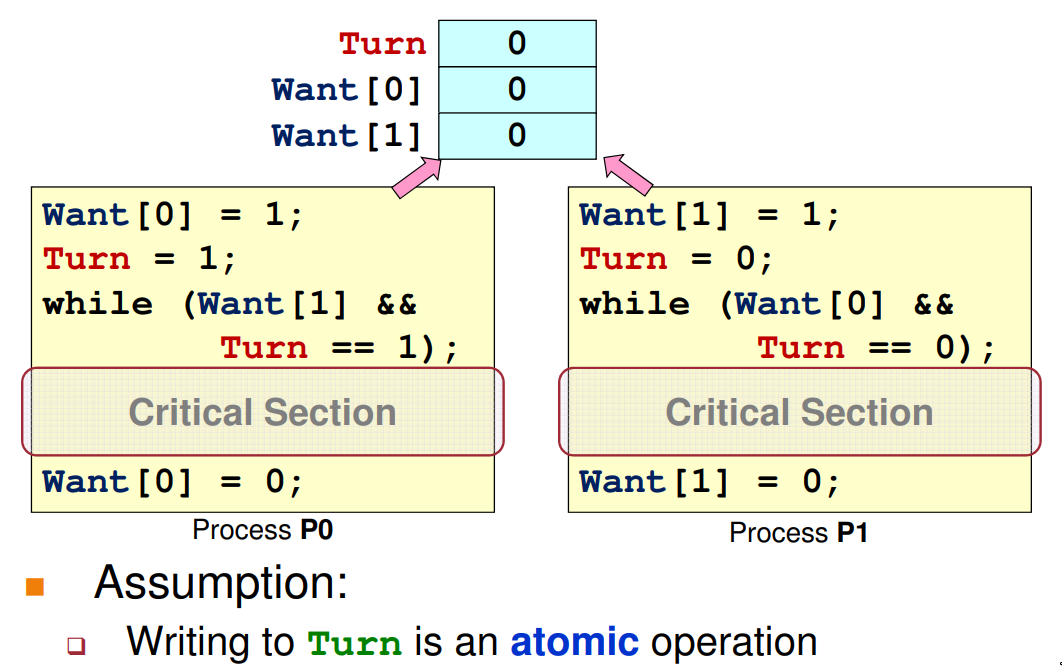
\includegraphics[width=0.24\textwidth]{peterson_algorithm}
        \end{center}
        Disadvantages
        \ull {
          \item Busy waiting: Using CPU cycles to wait for something to happen
          \item Low level implementation
          \item Not general
        }
      \paragraph{Test and Set}
        \ull {
          \item \ic{TestAndSet Register, MemoryLocation}
          \item Single atomic machine operation, even in multi-core systems
          \item Loads current content at MemoryLocation to Register, then stores a 1 into MemoryLocation
          \item \ic{while(TestAndSet(MemoryLocation) == 1);}
          \item Only if you locked it, you will get 0
        }
    \subsection*{Semaphores}
      \paragraph{\ic{Wait(S)}}
        \ull {
          \item If S $\leq 0$, blocks
          \item Decrement S
          \item Also known as \ic{P()} or \ic{Down()}
        }
      \paragraph{\ic{Signal(S)}}
        \ull {
          \item Increment S
          \item Wakes up one sleeping process (if any)
          \item Never blocks
          \item Also known as \ic{V()} or \ic{Up()}
        }
      \paragraph{Invariant}
        Given $S_\text{initial} \geq 0$,
        \[ S_\text{current} = S_\text{initial} + N_\text{signal} - N_\text{wait} \]
        \ull {
          \item $N_\text{signal}$: number of \ic{signal()} operations executed
          \item $N_\text{wait}$: number of \ic{wait()} operations completed
        }
      \paragraph{Variants}
        \ull {
          \item Binary semaphore: $S = 0$ or 1
          \item General (counting) semaphore: $S \geq 0$
          \item General semaphore can be mimicked by binary semaphores
        }
      \paragraph{Mutex}
        \ull {
          \item Implemented as a binary semaphore
          \item Invariant:
            \[ S_\text{current} + N_\text{CS} = 1 \]
        }
      \paragraph{Misc}
        \ull {
          \item Semaphore can be used to block process B until process A finishes executing a particular statement
          \item No unknown unsolvable synchronization problem with semaphore
          \item Alternative: conditional variable
          \item Always consider both single-core and multi-core systems
        }
\end{multicols*}
\end{document}
